\documentclass{standalone}
\usepackage{tikz}
\usepackage{bm}

\begin{document}
    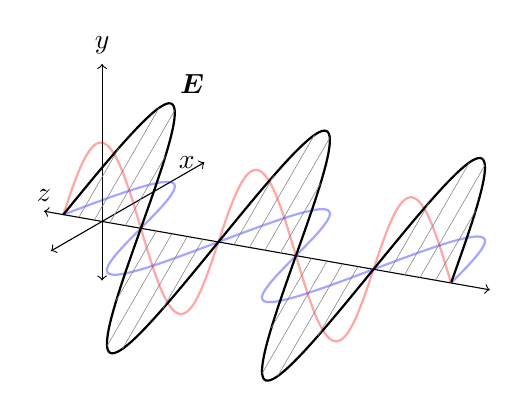
\begin{tikzpicture}[x={(-10:1cm)},y={(90:1cm)},z={(210:1cm)}]
        % Axes
        \draw[<->] (-0.75,0,0) node[above] {$z$} -- (5,0,0);
        \draw[<->] (0,-0.75,0) -- (0,2,0) node[above] {$y$};
        \draw[<->] (0,0,0.75) -- (0,0,-1.5) node[left] {$x$};
        % Propagation
        %\draw[->,ultra thick] (2.5,2,0) -- node[above] {$c/n$} (3.5,2,0);
        % Waves
        \draw[red,thick,opacity=0.35] plot[domain=-0.5:4.5,samples=200] (\x,{cos(deg(pi*\x))},0);
        \draw[blue,thick,opacity=0.35] plot[domain=-0.5:4.5,samples=200] (\x,0,-{cos(deg(pi*\x))});
        \draw[black,thick] plot[domain=-0.5:4.5,samples=200] (\x,{cos(deg(pi*\x))},-{cos(deg(pi*\x))});
        % Arrows
        \foreach \x in {-0.5,-0.3,...,4.4} {
          \draw[-, help lines] (\x,0,0) -- (\x,{cos(deg(pi*\x))},-{cos(deg(pi*\x))});
        }
        % Labels
        \node[above right] at (0,1,-1) {$\bm{E}$};
    \end{tikzpicture}
\end{document}